\documentclass{report}
\usepackage{graphicx} % Required for inserting images
\usepackage[a4paper, total={6in, 9in}]{geometry}
\usepackage{amsmath}
\usepackage{enumitem}
\usepackage{minted}
\usepackage{hyperref}
\hypersetup{
    colorlinks=true,
    linkcolor=blue,
    filecolor=magenta,      
    urlcolor=cyan,
    pdftitle={Fast Fourier transform}
    }

\begin{document}

\tableofcontents

\newpage
\chapter{Discovery}
Let's consider product of two \(d\) degree polynomials \(A(x)\) & \(B(x)\) is \(C(x)\).
\begin{math}
	
	A(x) = a_0 + a_1x + a_2x^2 + \ldots + a_{d-1}x^{d-1} + a_dx^d \\
	B(x) = b_0 + b_1x + b_2x^2 + \ldots + b_{d-1}x^{d-1} + b_dx^d \\
	C(x) = c_0 + c_1x + c_2x^2 + \ldots + c_{2d-1}x^{2d-1} + c_{2d}x^{2d}
\end{math}

The coefficients of \(C(x)\) can be calculated as follows:
\begin{math}
	c_k = \sum_{i=0}^{k} a_ib_{k-i} \quad \text{for} \quad k = 0, 1, 2, \ldots, 2d
\end{math}

This calculation requires \(O(d^2)\) operations. Can we do better?

\section{Convolution}
The product of two polynomials is called the convolution of the two coefficient sequences. The convolution of two sequences \(a_0, a_1, \ldots, a_{d-1}\) and \(b_0, b_1, \ldots, b_{d-1}\) is the sequence \(c_0, c_1, \ldots, c_{2d-1}\) where
\begin{math}
	c_k = \sum_{i=0}^{k} a_ib_{k-i} \quad \text{for} \quad k = 0, 1, 2, \ldots, 2d-1
\end{math}

The convolution of two sequences can be calculated in \(O(d^2)\) operations. Can we do better?

\section{Value  Representation}

The polynomial \(A(x)\) can be represented as a sequence of its values at \(d+1\) distinct points. For example, the polynomial \(A(x) = 3 + 4x + 5x^2\) can be represented as the sequence \((3, 7, 23)\) because \(A(0) = 3\), \(A(1) = 7\), and \(A(2) = 23\). The polynomial \(B(x)\) can also be represented as a sequence of its values at \(d+1\) distinct points. The product of two polynomials can be represented as the convolution of the two sequences of values.

We can calculate the convolution of two sequences of values in \(O(d)\) operations. So, we want to convert the coefficients of the polynomials to the values of the polynomials at \(d+1\) distinct points. This can be done using the Fast Fourier Transform (FFT).

\section{Coefficient to Value Representation}
To get \(d+1\) distinct points, we can use the \(d+1\) roots of unity. The \(d+1\) roots of unity are the complex numbers \(1, \omega, \omega^2, \ldots, \omega^d\) where \(\omega = e^{2\pi i/(d+1)}\). The polynomial \(A(x)\) can be represented as the sequence \(A(1), A(\omega), A(\omega^2), \ldots, A(\omega^d)\). The polynomial \(B(x)\) can also be represented as the sequence \(B(1), B(\omega), B(\omega^2), \ldots, B(\omega^d)\). The product of two polynomials can be represented as the convolution of the two sequences of values.


\section{What's the problem}
Now, we have the domain of the polynomials as the \(d+1\) roots of unity. But as we need to evaluate the value representation of each of the polynomial at \(d+1\) distinct points, this is still \(O(d^2)\). Can we do better? 

\section{Solution: even function}
We can divide the polynomial into two parts: the even terms and the odd terms. The even terms are the terms with even powers of \(x\) and the odd terms are the terms with odd powers of \(x\). For example, 



    
	$$A(x) = a_0 + a_1x + a_2x^2 + a_3x^3 + a_4x^4 + a_5x^5 + a_6x^6 + a_7x^7$$
	$$ = (a_0 + a_2x^2 + a_4x^4 + a_6x^6) + x(a_1 + a_3x^2 + a_5x^4 + a_7x^6)$$
	$$ =  (a_0 + a_2x^2 + a_4x^4 + a_6x^6) + x(a_0 + a_2x^2 + a_4x^4 + a_6x^6)x $$
	$$A(x)= A_e(x^2) + xA_o(x^2)$$
	$$A(x_i) = A_e(x_i^2) + x_iA_o(x_i^2)$$
	$$A(-x_i) = A_e(x_i^2) - x_iA_o(x_i^2)$$

here, \(A_e(x)\) is the polynomial with the even terms and \(A_o(x)\) is the polynomial with the odd terms. Now, both \(A_e(x)\) and \(A_o(x)\) are of degree \(d/2\). 
As both \(A_e(x)\) and \(A_o(x)\) are functions of \(x^2\), we can evaluate \(A(x)\) using \pm pairs of points. Hence, we need to evaluate \(A_e(x)\) and \(A_o(x)\) at \(d/2 + 1\) distinct points. Improvement!!

\section{Generalization}
We can generalize this to any degree polynomial.
For a \(n-1\) degree polynomial, 

$$	P(x) = a_0 + a_1x + a_2x^2 + \ldots + a_{n-1}x^{n-1} $$
we need to evaluate \(P(x)\) at \(n\) distinct points. $\pm x_1,\pm x_2, \ldots, \pm x_n $

$$ P(x) = P_e(x^2) + xP_o(x^2)$$
$$ P(x_i) = P_e(x_i^2) + x_iP_o(x_i^2)$$
 $$P(-x_i) = P_e(x_i^2) - x_iP_o(x_i^2)$$

\(P_e(x^2)\) and \(P_o(x^2)\) are of degree \(n/2-1\).\newline
So, we need to evaluate both \(P_e(x^2)\) and \(P_o(x^2)\) at $ x_1^2, x_2^2, \ldots, x_{n/2}^2 (n/2 + 1 \text{ points.})$ \newline
This is the start of a recursive algorithm to evaluate a polynomial at \(n\) distinct points.

\section{Divide and Conquer}
Now we have a recursive algorithm to evaluate a polynomial at \(n\) distinct points. We can use the divide and conquer paradigm to evaluate the polynomial at \(n\) distinct points.In each step, We can divide the polynomial into two parts: the even terms and the odd terms. We can evaluate the even and odd terms at \(n/2 + 1\) distinct points. This is the divide step. We can then combine the results of the even and odd terms to get the result for the entire polynomial. This is the conquer step. As the polynomial is divided into two parts at each step, the depth of the recursion is \(O(\log n)\). The time complexity of the algorithm is \(O(n \log n)\).

\section{Another Problem}
In the first step divide and conquer algorithm, we have squared the $x$ in the polynomial. So, we don't have the $\pm$ pairs in the very second step of the algorithm. It means, the recursion will break! We need to find a way to get the$ \pm $ pairs in the very second step of the algorithm. Or a way where we can get the $\pm $pairs after squaring the \(x\).

\section{Solution: Roots of Unity}
We can solve the problem of getting negative number after squaring the \(x\) by using the \(n\) roots of unity. The \(n\) roots of unity are the complex numbers \(1, \omega, \omega^2, \ldots, \omega^{n-1}\) where \(\omega = e^{2\pi i/n}\). 
So, for a polynomial of degree \(d\), we need \(n \geq d + 1\) points to evaluate where $n = 2^k , k \epsilon   \mathbb{Z} $ .


\section{Why does this work?}
For any of $j$th root of unity $\omega^j = - \omega^{j + n/2} \implies (\omega^j and -\omega^j)$ are $\pm$ pairs.
\centering
	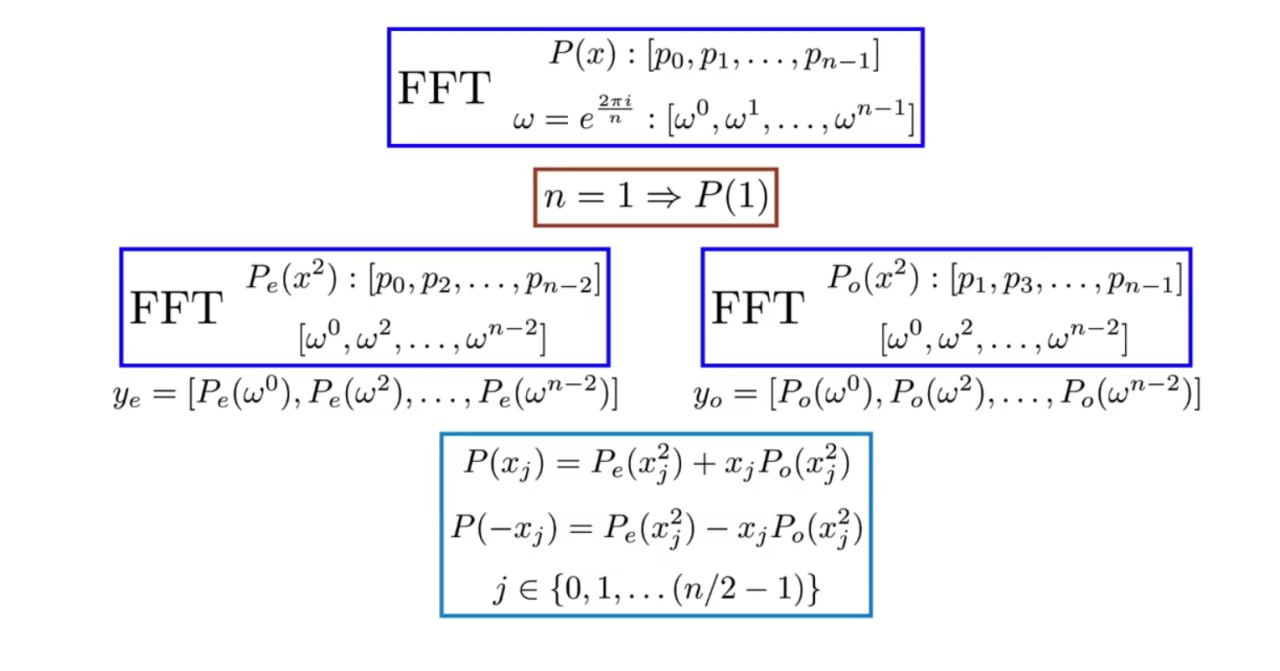
\includegraphics[width=\textwidth]{imp1.jpg}







\end{document}